% Created by tikzDevice version 0.12.6 on 2024-01-22 14:41:40
% !TEX encoding = UTF-8 Unicode
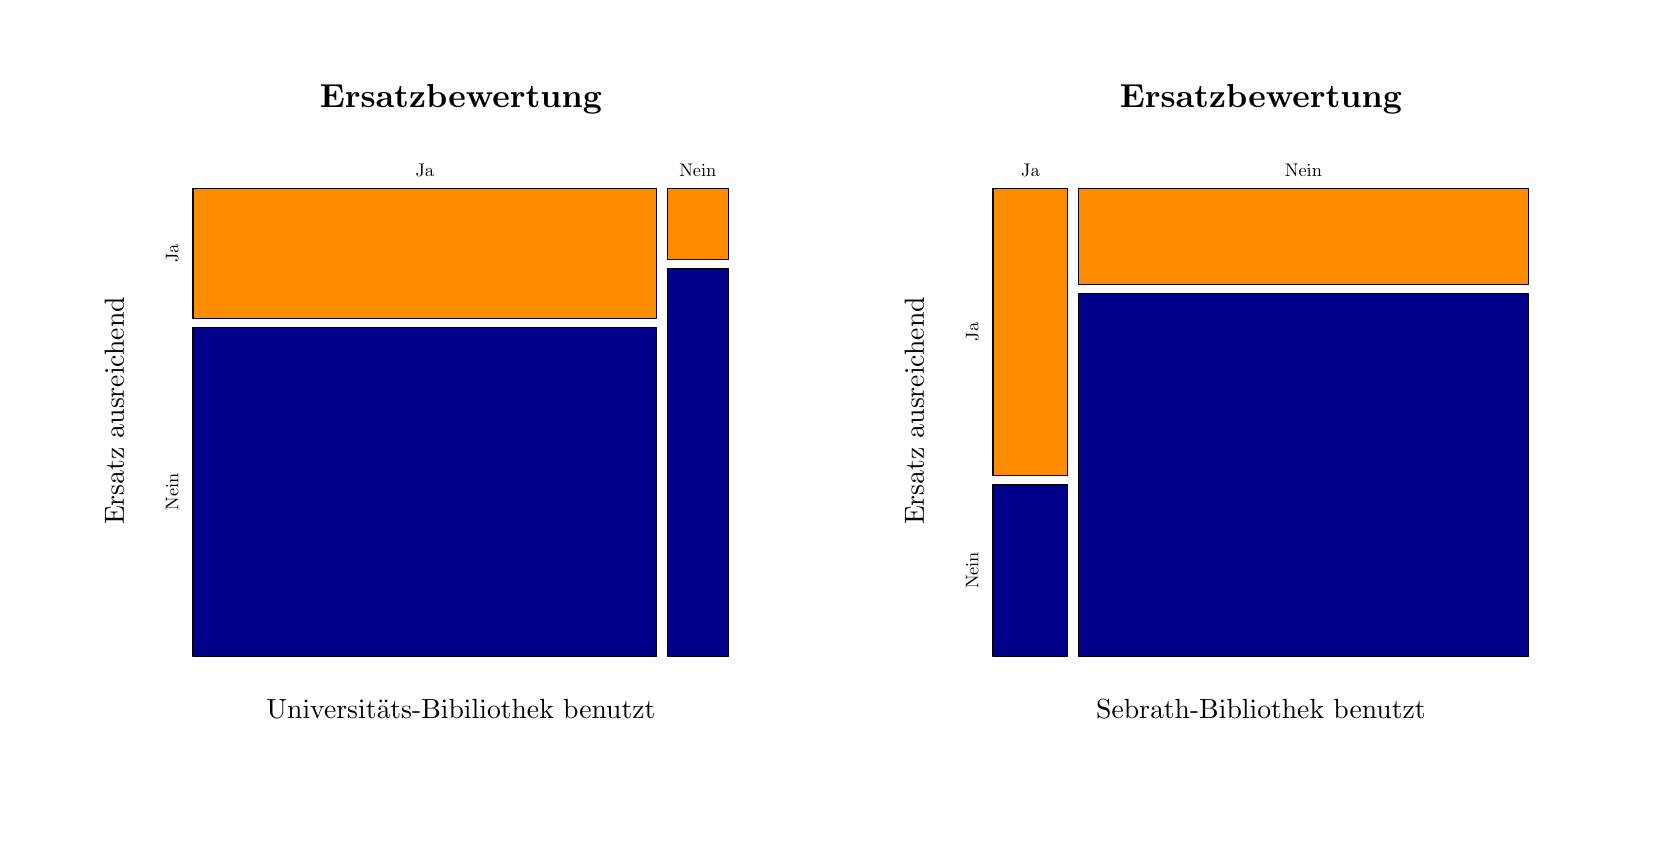
\begin{tikzpicture}[x=1pt,y=1pt]
\definecolor{fillColor}{RGB}{255,255,255}
\path[use as bounding box,fill=fillColor,fill opacity=0.00] (0,0) rectangle (578.16,289.08);
\begin{scope}
\path[clip] (  0.00,  0.00) rectangle (289.08,289.08);
\definecolor{drawColor}{RGB}{0,0,0}

\node[text=drawColor,anchor=base,inner sep=0pt, outer sep=0pt, scale=  1.20] at (156.54,260.34) {\bfseries Ersatzbewertung};

\node[text=drawColor,anchor=base,inner sep=0pt, outer sep=0pt, scale=  1.00] at (156.54, 39.60) {Universitäts-Bibiliothek benutzt};

\node[text=drawColor,rotate= 90.00,anchor=base,inner sep=0pt, outer sep=0pt, scale=  1.00] at ( 34.80,150.54) {Ersatz ausreichend};
\end{scope}
\begin{scope}
\path[clip] (  0.00,  0.00) rectangle (578.16,289.08);
\definecolor{drawColor}{RGB}{0,0,0}

\node[text=drawColor,anchor=base,inner sep=0pt, outer sep=0pt, scale=  0.66] at (143.50,235.34) {Ja};

\node[text=drawColor,anchor=base,inner sep=0pt, outer sep=0pt, scale=  0.66] at (242.14,235.34) {Nein};

\node[text=drawColor,rotate= 90.00,anchor=base,inner sep=0pt, outer sep=0pt, scale=  0.66] at ( 54.48,207.51) {Ja};

\node[text=drawColor,rotate= 90.00,anchor=base,inner sep=0pt, outer sep=0pt, scale=  0.66] at ( 54.48,121.31) {Nein};
\end{scope}
\begin{scope}
\path[clip] ( 49.20, 61.20) rectangle (263.88,239.88);
\definecolor{drawColor}{RGB}{0,0,0}
\definecolor{fillColor}{RGB}{255,140,0}

\path[draw=drawColor,line width= 0.4pt,line join=round,line cap=round,fill=fillColor] ( 59.73,184.09) --
	(227.27,184.09) --
	(227.27,230.94) --
	( 59.73,230.94) --
	cycle;
\definecolor{fillColor}{RGB}{0,0,139}

\path[draw=drawColor,line width= 0.4pt,line join=round,line cap=round,fill=fillColor] ( 59.73, 61.92) --
	(227.27, 61.92) --
	(227.27,180.71) --
	( 59.73,180.71) --
	cycle;
\definecolor{fillColor}{RGB}{255,140,0}

\path[draw=drawColor,line width= 0.4pt,line join=round,line cap=round,fill=fillColor] (231.14,205.45) --
	(253.14,205.45) --
	(253.14,230.94) --
	(231.14,230.94) --
	cycle;
\definecolor{fillColor}{RGB}{0,0,139}

\path[draw=drawColor,line width= 0.4pt,line join=round,line cap=round,fill=fillColor] (231.14, 61.92) --
	(253.14, 61.92) --
	(253.14,202.07) --
	(231.14,202.07) --
	cycle;
\end{scope}
\begin{scope}
\path[clip] (289.08,  0.00) rectangle (578.16,289.08);
\definecolor{drawColor}{RGB}{0,0,0}

\node[text=drawColor,anchor=base,inner sep=0pt, outer sep=0pt, scale=  1.20] at (445.62,260.34) {\bfseries Ersatzbewertung};

\node[text=drawColor,anchor=base,inner sep=0pt, outer sep=0pt, scale=  1.00] at (445.62, 39.60) {Sebrath-Bibliothek benutzt};

\node[text=drawColor,rotate= 90.00,anchor=base,inner sep=0pt, outer sep=0pt, scale=  1.00] at (323.88,150.54) {Ersatz ausreichend};
\end{scope}
\begin{scope}
\path[clip] (  0.00,  0.00) rectangle (578.16,289.08);
\definecolor{drawColor}{RGB}{0,0,0}

\node[text=drawColor,anchor=base,inner sep=0pt, outer sep=0pt, scale=  0.66] at (362.35,235.34) {Ja};

\node[text=drawColor,anchor=base,inner sep=0pt, outer sep=0pt, scale=  0.66] at (460.98,235.34) {Nein};

\node[text=drawColor,rotate= 90.00,anchor=base,inner sep=0pt, outer sep=0pt, scale=  0.66] at (343.56,179.17) {Ja};

\node[text=drawColor,rotate= 90.00,anchor=base,inner sep=0pt, outer sep=0pt, scale=  0.66] at (343.56, 92.97) {Nein};
\end{scope}
\begin{scope}
\path[clip] (338.28, 61.20) rectangle (552.96,239.88);
\definecolor{drawColor}{RGB}{0,0,0}
\definecolor{fillColor}{RGB}{255,140,0}

\path[draw=drawColor,line width= 0.4pt,line join=round,line cap=round,fill=fillColor] (348.81,127.41) --
	(375.89,127.41) --
	(375.89,230.94) --
	(348.81,230.94) --
	cycle;
\definecolor{fillColor}{RGB}{0,0,139}

\path[draw=drawColor,line width= 0.4pt,line join=round,line cap=round,fill=fillColor] (348.81, 61.92) --
	(375.89, 61.92) --
	(375.89,124.03) --
	(348.81,124.03) --
	cycle;
\definecolor{fillColor}{RGB}{255,140,0}

\path[draw=drawColor,line width= 0.4pt,line join=round,line cap=round,fill=fillColor] (379.75,196.43) --
	(542.22,196.43) --
	(542.22,230.94) --
	(379.75,230.94) --
	cycle;
\definecolor{fillColor}{RGB}{0,0,139}

\path[draw=drawColor,line width= 0.4pt,line join=round,line cap=round,fill=fillColor] (379.75, 61.92) --
	(542.22, 61.92) --
	(542.22,193.05) --
	(379.75,193.05) --
	cycle;
\end{scope}
\end{tikzpicture}
